\section{Synchronmaschine}
    \renewcommand{\arraystretch}{2.5} 
\begin{minipage}{0.5\linewidth}   
\textcolor{green}{Vorteil}:
\begin{itemize} 
	\item sehr robust, elektrodynamisch, mechanisch und thermisch stabil
    \item Hoher Wirkungsgrad (80-90\%)
	\item Drehmoment einfach bestimmbar
	\item Einfache Konstruktion
	\item Man kann Blindleistung mit diesem Motor kompensieren
\end{itemize}
\textcolor{red}{Nachteil}:
\begin{itemize}
\item hoher Anlaufstrom
\end{itemize}
\end{minipage}
\begin{minipage}{0.33\linewidth}
    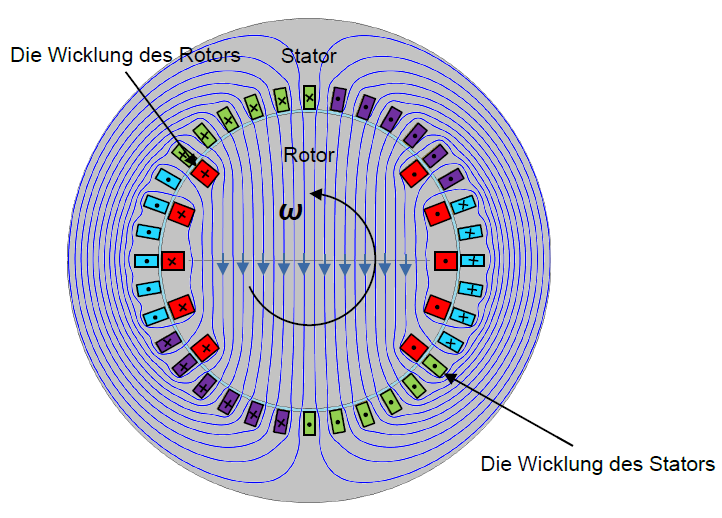
\includegraphics[width = 8cm]{images/AufbauSynchronmotor}
\end{minipage}
\\
\subsection{Funktionsweise}
Das Drehfeld und der Rotor einer Synchronmaschine rotieren mit derselben Geschwindigkeit d.h. sind sie im Synchronlauf. \\
\textbf{Anwendung:} zur Umwandlung von mechanischer Energie in elektrische Energie.

\subsection{Aufbau und Wirkungsprinzip}
    \begin{minipage}[b]{0.5\linewidth}
    	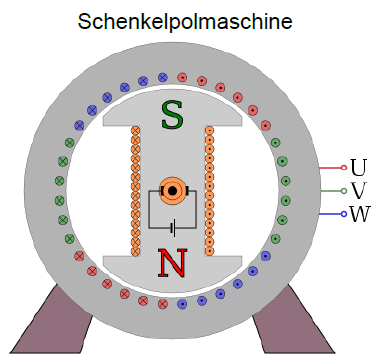
\includegraphics[width = 5cm]{images/Schenkelpolmaschine}
    \end{minipage}
    \begin{minipage}[b]{0.5\linewidth}
    	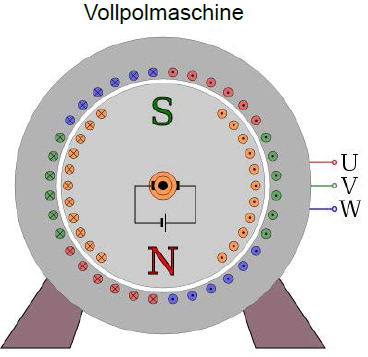
\includegraphics[width = 5cm]{images/Vollpolmaschine}
    \end{minipage}
    Folgende Eigenschaften gelten für grosse Generatoren >1GW darunter können die Bauarten beliebig sein.
    \begin{tabular}[b]{| C{0.4\linewidth} | C{0.4\linewidth} |}
    	\hline
    	\textbf{Schenkelpolmaschine} &
        \textbf{Vollpolmaschine}
        \\ \hline
        
    	\vspace{-0.7cm}
    	\begin{itemize}
            \item Wasserkraftwerk
    		\item Grössere Polpaarzahl
    		\item Kleinere Drehzahl
    	\end{itemize} &
        \vspace{-0.7cm}
        \begin{itemize}
            \item Wärmekraftwerke
            \item Polpaarzahl = 1
        	\item Grössere Drehzahl
        \end{itemize}
        \\ \hline
    \end{tabular}
    \\
    \clearpage
    \pagebreak


    \begin{minipage}[b]{0.5\linewidth}
        \subsection{Grundgleichungen}
        \textbf{Strang Ersatzschaltung:}\newline
        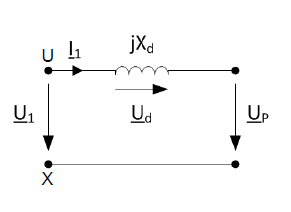
\includegraphics[width = 6cm]{images/Wicklung1}
    \end{minipage}
    \begin{minipage}[t]{0.5\linewidth}
        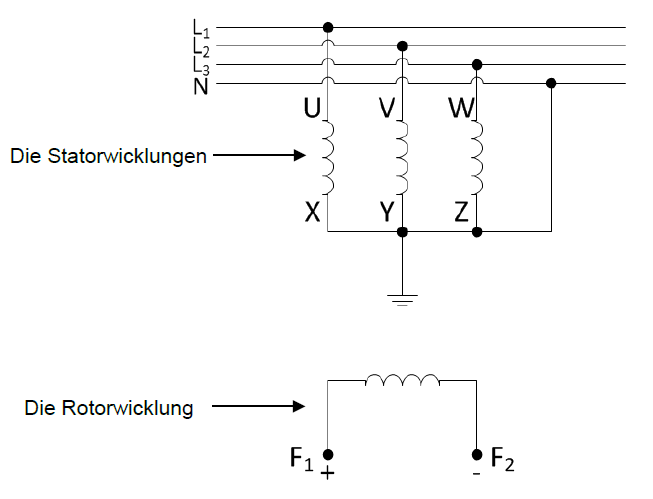
\includegraphics[width = 7.5cm]{images/Wicklungen}
    \end{minipage}
    \vspace{-1cm}
    \begin{longtable}[b]{| C{5cm}| P{8.5cm} | P{5 cm} |}
    	\hline
        \textbf{Strangspannung} 	&
        $\underline{U_1\!} = \underline{U_d\!} + \underline{U_P\!}$ &
        $U_P \, \widehat{=}$ der Polradspannung
        \\ \hline
        
        \textbf{Spulenspannung}	&
        $\underline{U_d} = jX_d\cdot \underline{I_1}$ &
        \\ \hline
        
        \textbf{Polradspannung} \newline (fiktive Hilfsgrösse) &
        $\underline{U_P} = \underline{U_P}\left(I_e\right)$ \newline\newline
        $\underline{U_P} = jX_h\cdot I_{e}\,'$  &
        $I_e \, \widehat{=}$ dem Erregerstrom \newline
        $I_e \,' \widehat{=}$ dem Erregerstrom umgerechnet auf die Statorseite
        \\ \hline
        
        \textbf{Synchronreaktanz} &
        $X_d = X_{\sigma 1} + X_h$ \newline \newline 
        $X_d = 2\pi f L_d$ \newline \newline
        $X_d = \dfrac{U_{1Str}}{I_K}$&
        $X_d \, \widehat{=} $ Synchronreaktanz \newline
        $X_{\sigma 1} \, \widehat{=}$ Streureaktanz des Stators \newline
        $X_h \, \widehat{=}$ der Hauptreaktanz \newline 
        $U_1\, \widehat{=}$ der Verketteten Spannung
        \\ \hline
        
        \textbf{Leistung} \newline 
        \tabbild[scale=0.4]{images/SynchronKennlinie} &
        $\cos(\varphi) = -\sin(\alpha) $ \newline\newline
       	$ (X_d \cdot I_{1Str})^2=U_{1Str}^2+U_{pStr}^2 - 2\cdot U_{1Str}\cdot U_{pStr}\cdot cos(\delta) $ \newline \newline
       	$P_{Str} = U_{Str}\cdot I_{Str}\cdot cos(\varphi)$ \newline
        \textcolor{red}{d} = $-U_p\cdot\sin(\delta)$ \newline
        \qquad $= X_d\cdot I_1\cdot\sin(\alpha) = -X_d\cdot I_1\cdot\cos(\varphi)$ \newline \newline
        $P(\delta) = 3\cdot P_{Str}(\delta)= 3\cdot\dfrac{U_{PStr}\cdot U_{1Str}}{X_d}\cdot\sin(\delta)$ \newline
        \textbf{Generatorbetrieb:} $\delta < 0$ \newline
        $P(\delta) = P_{mech}-P_V = \omega\cdot M - P_V$ \newline
        \textbf{Motorbetrieb:} $\delta > 0$ \newline
        $P(\delta) = P_{mech} + P_V = \omega\cdot M + P_V$ &
         $\varphi = -\alpha - 90^\degree   \quad\left[ grad \right]$ \newline \newline
        Polradwinkel $\delta =  \measuredangle (U_p, U_1)$  \newline \newline
        $U_P$ ist die Polradspannung, sie entspricht einer fiktiven Grösse! Sie kann wiederum durch ein Zeigerdiagramm bestimmt werden.\newline\newline
        \textbf{ Achte auf Y-$ \Delta $-Umrechnug} \newline
        Seite: \pageref{SternDreieck}
        \\ \hline
		\textbf{Erreger-Regulierkennlinien} & 
		$ \dfrac{I_e}{I_{e0}} = \sqrt{cos^2(\varphi) + \left(x\cdot\dfrac{I_1}{I_N}-sin(\varphi)\right)^2}$ &
        $I_e = f(I_1)$ \newline $cos(\varphi)$ gegeben \newline $I_1$ - gewünschter Netzstrom \newline Bezugswert $x = \dfrac{X_d}{X_N}$ \newline $ X_N = Normiert $
		\\ \hline
		\textbf{mechanisches Moment} &  $P = \Omega\cdot M = \dfrac{\omega}{p}\cdot M$ & Gilt falls $P_V = 0$ 
		\\ \hline	
	    \end{longtable}
    
    \begin{minipage}{0.5\linewidth}
        $ cos(\varphi) = x_{ind} \rightarrow \varphi^\degree >0 $ Strom eilt der Spannung nach\newline
        $ cos(\varphi) = x_{kap} \rightarrow \varphi^\degree <0 $ Strom eilt der Spannung voraus\newline
    \end{minipage}
\subsection{Zeigerdiagramm im Motorbetrieb}
    P > 0 und $\delta$ > 0 \newline \newline
    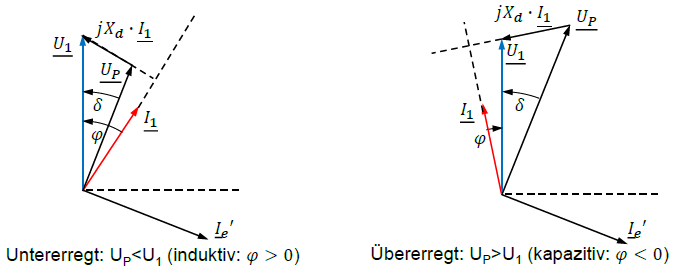
\includegraphics[width = 14 cm]{images/ZeigerdiagrammSynchronmaschine}

\subsection{Zeigerdiagramm im Generatorbetrieb}
    P < 0, $\delta$ < 0  \newline
    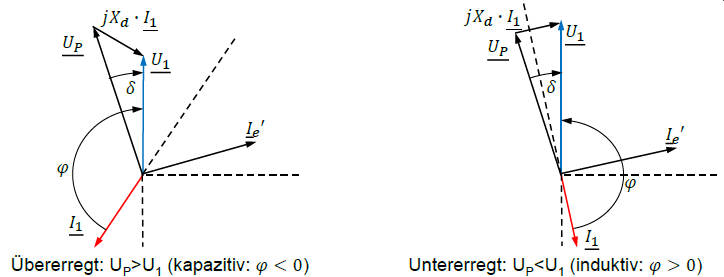
\includegraphics[width = 14 cm]{images/ZeigerdiagrammGeneratorbetrieb} \newline \newline
    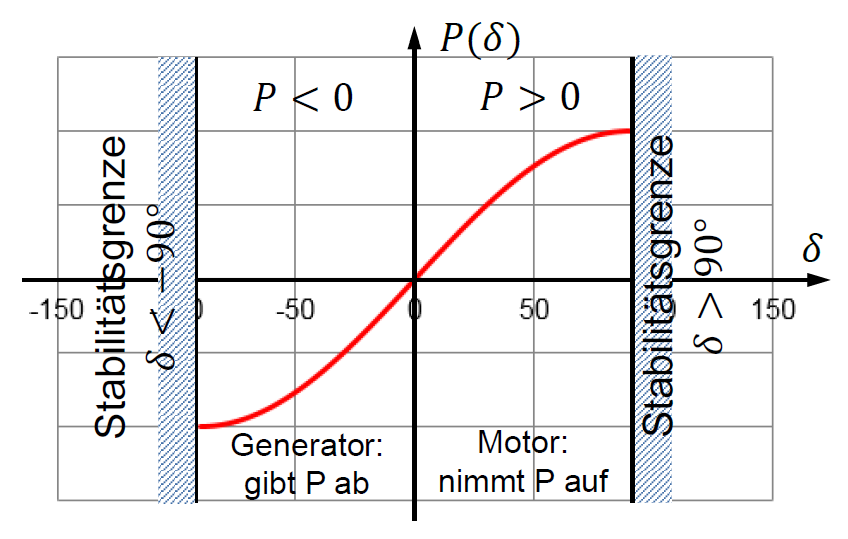
\includegraphics[scale = 0.35]{images/Stabilitaet}
    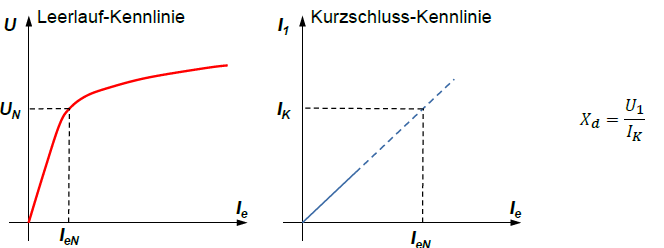
\includegraphics[scale = 0.7]{images/KennlinieSynchronmaschine}
\clearpage
\pagebreak
